% slides/week06_information_theory.tex
% Semana 6 — Information Theory para Machine Learning

% =========================
% Metadata
% =========================
\title[Semana 6: Information Theory]{Semana 6 — Information Theory para Machine Learning}
\subtitle{Entropía, cross-entropy, KL divergence y su papel como loss}
\author{Curso de Machine Learning — UAQ (Matemáticas Aplicadas)}
%\institute{Libro base: \textit{Probabilistic Machine Learning: An Introduction} (Kevin P. Murphy)}
\date{Semana 6}

% =========================
% Helpers (avoid redefinition if provided by theme/macros)
% =========================
\providecommand{\key}[1]{\textbf{#1}}
\providecommand{\term}[1]{\textit{#1}}

% "Dónde vamos en el temario" helper.
% Usage: \temariobar{Teoría}{Lab NumPy}{Lab sklearn}{Entregable}
\providecommand{\temariobar}[4]{%
% (Opción A) Para ahorrar espacio, el bloque actual se indica en el pie
% usando \insertsectionhead. Este macro se deja como no-op para no tener
% que borrarlo de todos los frames.
}

% =========================================================
% Indicador del bloque actual (Teoría / Lab / Entregable) en el pie
% =========================================================
\setbeamertemplate{headline}{}
\setbeamertemplate{footline}{%
  \leavevmode%
  \hbox{%
    \begin{beamercolorbox}[wd=.84\paperwidth,ht=2.25ex,dp=1ex,leftskip=1em]{author in head/foot}%
      \usebeamerfont{author in head/foot}\insertsectionhead
    \end{beamercolorbox}%
    \begin{beamercolorbox}[wd=.16\paperwidth,ht=2.25ex,dp=1ex,center]{date in head/foot}%
      \usebeamerfont{date in head/foot}\insertframenumber/\inserttotalframenumber
    \end{beamercolorbox}%
  }%
  \vskip0pt%
}

% Auto-outline at each section start — debe redefinirse por semana (el hook es global en Beamer).
\AtBeginSection[]{
  \begin{frame}{Semana 6 — mapa del temario (progreso)}
  \temariobar{Teoría}{Lab NumPy}{Lab sklearn}{Entregable}
  \vspace{0.3em}
  \begin{columns}[t]
  \column{0.5\textwidth}
  \begin{itemize}
    \item \textbf{Teoría}
    \item \textbf{Lab NumPy}
    \item \textbf{Lab sklearn}
  \end{itemize}
  \column{0.5\textwidth}
  \begin{itemize}
    \item \textbf{Entregable}
  \end{itemize}
  \end{columns}
  \end{frame}
}

% =========================================================
% PART: WEEK 6
% =========================================================
\part{Semana 6}

% =========================================================
% TITLE
% =========================================================
\begin{frame}
  \titlepage
\end{frame}

% =========================================================
% LECTURAS SUGERIDAS
% =========================================================
\begin{frame}{Lecturas sugeridas (para estos temas)}
\temariobar{\textbf{Teoría}}{Lab NumPy}{Lab sklearn}{Entregable}
\begin{itemize}
  \item \key{Capítulo 6 — Information theory}
  \begin{itemize}
    \item \key{6.1} Entropy
    \begin{itemize}
      \item \key{6.1.1} Entropy for discrete random variables
      \item \key{6.1.2} Cross entropy
      \item \key{6.1.3--6.1.5} Joint / conditional entropy, perplexity
    \end{itemize}
    \item \key{6.2} Relative entropy (KL divergence)
    \begin{itemize}
      \item \key{6.2.1--6.2.6} Definición, interpretación, no-negatividad, KL y MLE
    \end{itemize}
  \end{itemize}
\end{itemize}
\end{frame}

% =========================================================
% TEMARIO MAP
% =========================================================
\begin{frame}{Temario de la Semana 6 (qué cubrimos hoy)}
\temariobar{\textbf{Teoría}}{Lab NumPy}{Lab sklearn}{Entregable}
\begin{itemize}
  \item \textbf{Teoría (PML)}
  \begin{itemize}\small
    \item \key{1) Surprisal:} \(I(x)=-\log p(x)\), unidades (bits/nats) \hfill \key{(6.1.1)}
    \item \key{2) Entropía:} \(H(X)\) como incertidumbre promedio; ejemplos discretos \hfill \key{(6.1.1)}
    \item \key{3) Cross-entropy:} \(H(p,q)\), interpretación codificación / modelo \hfill \key{(6.1.2)}
    \item \key{4) KL:} \(\mathrm{KL}(p\|q)\), no-negatividad, orden \(p\) vs \(q\) \hfill \key{(6.2)}
    \item \key{5) Identidad:} \(H(p,q)=H(p)+\mathrm{KL}(p\|q)\) \hfill \key{(6.1.2, 6.2)}
    \item \key{6) ML:} CE/NLL en etiquetas one-hot, enlace con MLE e incertidumbre del modelo \hfill \key{(6.1.2, 6.2)}
  \end{itemize}
  \item \textbf{Lab NumPy}
  \begin{itemize}\small
    \item Calcular \(H(p)\), \(H(p,q)\) y \(\mathrm{KL}(p\|q)\) a mano en ejemplos pequeños
    \item Curva de entropía Bernoulli \(H(\theta)\); verificar casos límite numéricamente
  \end{itemize}
  \item \textbf{Lab sklearn}
  \begin{itemize}\small
    \item \texttt{log\_loss} y equivalencia con CE promedio en clasificación
    \item Comparar CE manual vs implementación en un mini-dataset
  \end{itemize}
  \item \textbf{Entregable}
\end{itemize}
\end{frame}

\begin{frame}{Hilo conductor: de “evaluar aciertos” a “evaluar probabilidades”}
\temariobar{\textbf{Teoría}}{Lab NumPy}{Lab sklearn}{Entregable}
\begin{itemize}
  \item Semana 5: métricas de clasificación y curvas ROC/PR miden, sobre todo, \key{decisiones} y \key{aciertos} bajo umbrales.
  \item Semana 6: si el modelo entrega una \textbf{distribución} \(\hat p(y\mid x)\), necesitamos una loss coherente con probabilidades.
  \item \key{Idea central:} surprisal \(\rightarrow\) entropía \(\rightarrow\) cross-entropy \(\rightarrow\) KL conectan incertidumbre, codificación y entrenamiento (MLE \(\equiv\) minimizar NLL/CE).
\end{itemize}
\end{frame}

% =========================================================
% SECTION: TEORÍA
% =========================================================
\section[Teoría]{Teoría\label{sec:teoria-w06}}

% =========================================================
% 1. PANORAMA DE LA SEMANA
% =========================================================
\subsection[Panorama]{Panorama de la semana}

\begin{frame}{¿Qué estudia information theory?}
\temariobar{\textbf{Teoría}}{Lab NumPy}{Lab sklearn}{Entregable}
\begin{itemize}
  \item \key{Pregunta central:} ¿cuánta incertidumbre hay en una fuente aleatoria y cuánto cuesta describir sus resultados?
  \item \key{Shannon (1948):} propone medidas cuantitativas para:
  \begin{itemize}
    \item la \textbf{incertidumbre} de una variable aleatoria,
    \item la \textbf{sorpresa} de observar un evento,
    \item el costo de usar un \textbf{modelo incorrecto} para describir los datos.
  \end{itemize}
  \item \key{Idea guía de la semana:} pasaremos de la sorpresa de un evento individual a la pérdida promedio de un modelo probabilístico.
  \item Esa ruta conceptual será:
  \[
    \text{surprisal} \;\longrightarrow\; \text{entropía} \;\longrightarrow\; \text{cross-entropy} \;\longrightarrow\; \mathrm{KL}.
  \]
\end{itemize}
\end{frame}

\begin{frame}{¿Por qué importa en machine learning?}
\temariobar{\textbf{Teoría}}{Lab NumPy}{Lab sklearn}{Entregable}
\begin{itemize}
  \item En muchos modelos de ML no solo queremos \textbf{predecir una clase}, sino asignar una \textbf{distribución de probabilidad} sobre las clases.
  \item Esto requiere una forma coherente de:
  \begin{itemize}
    \item medir la \textbf{incertidumbre} del modelo,
    \item \textbf{comparar} distribuciones (datos vs modelo),
    \item definir \textbf{funciones de pérdida} basadas en probabilidad.
  \end{itemize}
  \item Las cantidades de information theory (entropía, cross-entropy, divergencia KL) serán los ladrillos para:
  \begin{itemize}
    \item diseñar la loss estándar de clasificación,
    \item entender por qué maximizar likelihood equivale a minimizar NLL/CE,
    \item preparar métodos probabilísticos más avanzados.
  \end{itemize}
\end{itemize}
\end{frame}

% =========================================================
% 2. DESARROLLO CONCEPTUAL
% =========================================================
\subsection[Conceptos]{Desarrollo conceptual}

% -------------------- 2.1 Self-information --------------------
\subsection{Self-information / surprisal}

\begin{frame}{Self-information / surprisal: definición e intuición}
\temariobar{\textbf{Teoría}}{Lab NumPy}{Lab sklearn}{Entregable}
\begin{itemize}
  \item Sea un evento \(x\) con probabilidad \(p(x)\in(0,1]\).
  \item \key{Definición (Shannon):}
  \[
    I(x) \;\triangleq\; -\log p(x)
  \]
  \item \key{Unidades:}
  \begin{itemize}
    \item base 2 \(\Rightarrow\) bits,
    \item base \(e\) \(\Rightarrow\) nats.
  \end{itemize}
  \item \key{Intuición:}
  \begin{itemize}
    \item cuanto más improbable es \(x\), mayor es su sorpresa/información;
    \item si \(p(x)=1\) (evento seguro), entonces \(I(x)=0\): no hay sorpresa.
  \end{itemize}
\end{itemize}
\end{frame}

\begin{frame}{Ejemplo numérico de surprisal}
\temariobar{\textbf{Teoría}}{Lab NumPy}{Lab sklearn}{Entregable}
\begin{itemize}
  \item Evento A: lanzar una moneda justa y obtener cara.
  \[
    p(A)=0.5,\quad I(A) = -\log_2(0.5) = 1 \text{ bit}
  \]
  \item Evento B: lanzar un dado justo y obtener un 6.
  \[
    p(B)=\tfrac{1}{6},\quad I(B) = -\log_2\Big(\tfrac{1}{6}\Big)\approx 2.585 \text{ bits}
  \]
  \item \key{Lectura:} observar un 6 específico en un dado justo aporta más información que observar cara en una moneda justa.
\end{itemize}

\vspace{0.5em}
\textbf{Nota:}
Confundir “información” con “importancia” del evento. Un evento raro tiene mucha información en el sentido de sorpresa, no necesariamente en el sentido de relevancia práctica.
\end{frame}

\begin{frame}{Analogía útil para explicar surprisal}
\temariobar{\textbf{Teoría}}{Lab NumPy}{Lab sklearn}{Entregable}
\begin{itemize}
  \item Imagina un sistema de \textbf{alertas}:
  \begin{itemize}
    \item “Todo funciona normal” (muy frecuente) \(\rightarrow\) poca sorpresa.
    \item “El servidor crítico está caído” (muy raro) \(\rightarrow\) mucha sorpresa.
  \end{itemize}
  \item El valor \(I(x)\) mide “\textbf{cuán inesperado}” fue el evento.
  \item En ML, si el modelo asigna probabilidad muy baja a la clase verdadera, la loss será alta: el modelo se “sorprende” demasiado por lo que pasó en realidad.
\end{itemize}
\vspace{0.8em}
\begin{center}
\small
\begin{tabular}{lccc}
\toprule
 & Evento frecuente & Evento raro & Evento muy raro \\
\midrule
Probabilidad \(p(x)\) & 0.8 & 0.15 & 0.05 \\
Sorpresa \(I(x)=-\log_2 p(x)\) & \(\approx 0.32\) & \(\approx 2.74\) & \(\approx 4.32\) \\
\bottomrule
\end{tabular}
\end{center}
\end{frame}

% -------------------- 2.2 Entropy --------------------
\subsection{Entropía}

\begin{frame}{Entropía: definición formal}
\temariobar{\textbf{Teoría}}{Lab NumPy}{Lab sklearn}{Entregable}
\begin{itemize}
  \item Sea \(X\) una variable discreta con distribución \(p(x)\) sobre un conjunto finito \(\mathcal{X}\).
  \item \key{Definición de entropía de Shannon:}
  \[
    H(X) \;\triangleq\; -\sum_{x\in\mathcal{X}} p(x)\,\log p(x)
  \]
  \item \key{Interpretaciones equivalentes:}
  \begin{itemize}
    \item incertidumbre promedio de \(X\),
    \item información esperada de los eventos \(x\) (promedio de \(I(x)\)),
    \item longitud promedio mínima (en bits) de un código óptimo para \(X\).
  \end{itemize}
  \item \key{Notación alternativa:} \(H(p)\) cuando queremos enfatizar que depende de la distribución \(p\).
\end{itemize}
\end{frame}

\begin{frame}{Entropía como esperanza de surprisal}
\temariobar{\textbf{Teoría}}{Lab NumPy}{Lab sklearn}{Entregable}
\begin{itemize}
  \item Ya definimos la sorpresa de un evento individual:
  \[
    I(x)=-\log p(x).
  \]
  \item Si ahora \(X\sim p\), la sorpresa \textbf{promedio} es:
  \[
    \mathbb{E}_{p}[I(X)] = \sum_x p(x)\,I(x).
  \]
  \item Sustituyendo \(I(x)=-\log p(x)\):
  \[
    \mathbb{E}_{p}[I(X)] = \sum_x p(x)\,[-\log p(x)] = -\sum_x p(x)\log p(x).
  \]
  \item \key{Conclusión:}
  \[
    H(X)=\mathbb{E}_{p}[I(X)].
  \]
  \item Esta identidad conecta de forma natural evento individual \(\rightarrow\) incertidumbre promedio.
\end{itemize}
\end{frame}

\begin{frame}{Ejemplo: entropía de una distribución discreta simple}
\temariobar{\textbf{Teoría}}{Lab NumPy}{Lab sklearn}{Entregable}
\begin{itemize}
  \item Supón \(X\in\{a,b,c\}\) con:
  \[
    p(a)=0.5,\quad p(b)=0.25,\quad p(c)=0.25.
  \]
  \item Calculamos:
  \[
    H(X) = -\big[0.5\log_2 0.5 + 0.25\log_2 0.25 + 0.25\log_2 0.25\big].
  \]
  \item Paso a paso:
  \[
    \log_2 0.5 = -1,\quad \log_2 0.25=-2
  \]
  \[
    H(X) = -\big[0.5(-1) + 0.25(-2) + 0.25(-2)\big]
    = -\big[-0.5 -0.5 -0.5\big] = 1.5 \text{ bits.}
  \]
  \item \key{Lectura:} en promedio, “necesitamos” 1.5 bits para codificar \(X\) de forma óptima.
\end{itemize}
\end{frame}

\begin{frame}{Entropía y dispersión de la distribución}
\temariobar{\textbf{Teoría}}{Lab NumPy}{Lab sklearn}{Entregable}
\begin{itemize}
  \item Para un alfabeto fijo:
  \begin{itemize}
    \item la \textbf{entropía es máxima} cuando la distribución es uniforme (toda la probabilidad repartida por igual);
    \item la \textbf{entropía es mínima} (0) cuando la distribución es degenerada (toda la masa en un solo punto).
  \end{itemize}
  \item Intuición: cuanta más “dispersa” esté la probabilidad entre muchos valores plausibles, más incertidumbre tenemos; cuando casi todo el peso está en un único valor, apenas dudamos.
  \item \key{Mensaje para ML:} una predicción con probabilidades muy repartidas tiene mayor entropía que una predicción muy concentrada en una sola clase.
\end{itemize}
\end{frame}

\begin{frame}{Entropía de una moneda: visualización}
\temariobar{\textbf{Teoría}}{Lab NumPy}{Lab sklearn}{Entregable}
\begin{itemize}
  \item Para una moneda con parámetro \(\theta = \Pr(\text{cara})\), la entropía
  \[
    H(\theta) = -\theta\log_2\theta - (1-\theta)\log_2(1-\theta)
  \]
  mide cuánta incertidumbre hay antes de observar el resultado del lanzamiento.
  \item Analíticamente sabemos que:
  \begin{itemize}
    \item la incertidumbre es \textbf{máxima} en \(\theta=0.5\) (moneda justa),
    \item tiende a \(0\) cuando \(\theta\to 0\) o \(\theta\to 1\) (moneda casi determinista).
  \end{itemize}
  \item En la siguiente gráfica se ve claramente esta forma “en campana invertida” de \(H(\theta)\).
\end{itemize}
\end{frame}

\begin{frame}{Entropía de una moneda: curva \(H(\theta)\)}
\temariobar{\textbf{Teoría}}{Lab NumPy}{Lab sklearn}{Entregable}
\begin{center}
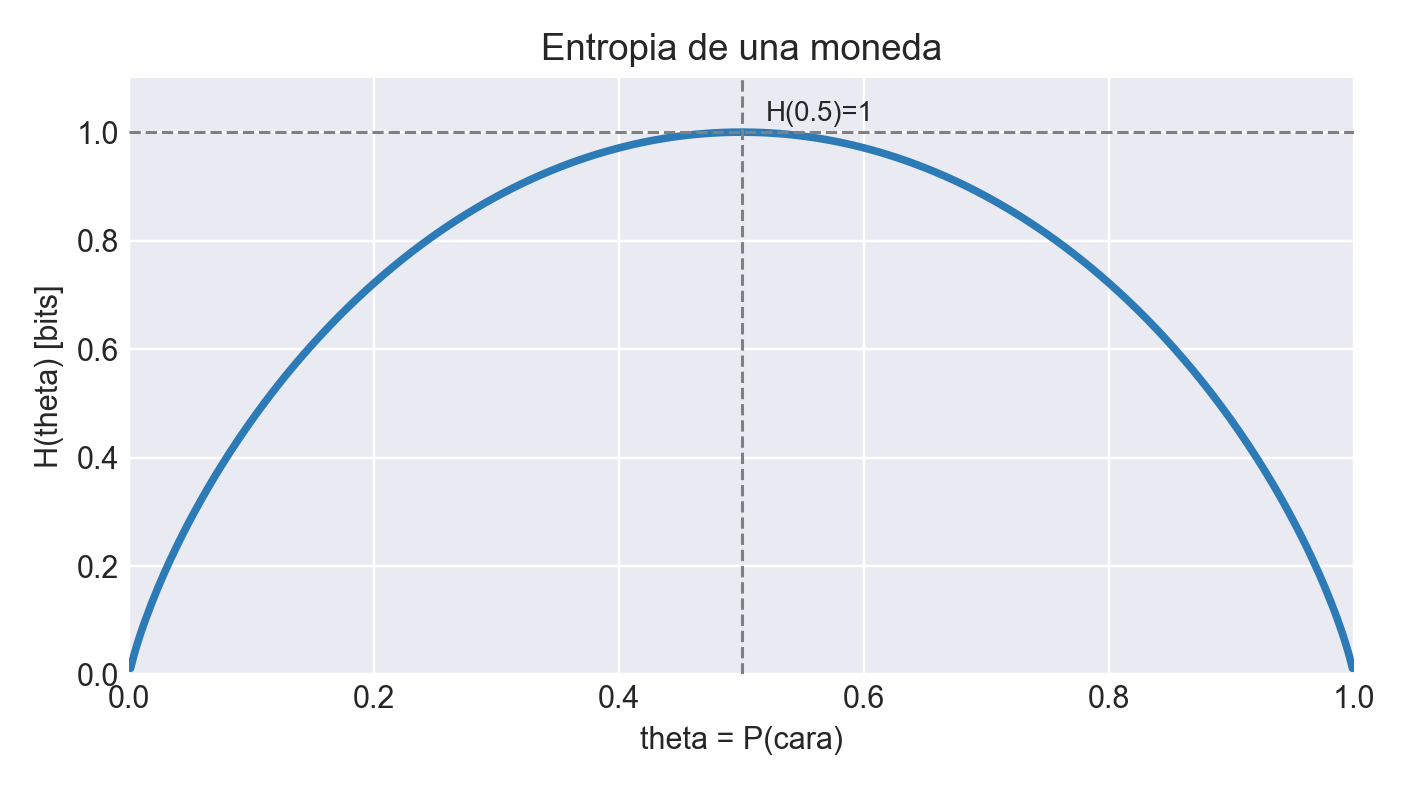
\includegraphics[width=0.7\textwidth,height=0.45\textheight,keepaspectratio]{slides/figs/week06_entropy_coin.png}
\end{center}
\vspace{0.5em}
\small
La entropía es máxima para \(\theta=0.5\) (moneda justa) y se aproxima a \(0\) cuando \(\theta\) se acerca a \(0\) o \(1\), es decir, cuando la moneda es prácticamente determinista.
\end{frame}

% -------------------- 2.3 Cross-entropy --------------------
\subsection{Cross-entropy}

\begin{frame}{Cross-entropy: definición e interpretación}
\temariobar{\textbf{Teoría}}{Lab NumPy}{Lab sklearn}{Entregable}
\begin{itemize}
  \item Tenemos una \textbf{distribución verdadera} \(p\) y un \textbf{modelo} \(q\).
  \item \key{Definición:}
  \[
    H(p,q) \;\triangleq\; -\sum_{x} p(x)\,\log q(x).
  \]
  \item \key{Lectura:}
  \begin{itemize}
    \item sorpresa promedio de datos generados por \(p\), pero evaluada con el modelo \(q\),
    \item costo promedio de codificar datos de \(p\) usando el código óptimo para \(q\).
  \end{itemize}
  \item Si \(q=p\), entonces \(H(p,q)=H(p)\): el mejor caso es usar el modelo verdadero.
\end{itemize}
\end{frame}

\begin{frame}{Ejemplo: cross-entropy entre dos distribuciones sobre \(\{a,b\}\)}
\temariobar{\textbf{Teoría}}{Lab NumPy}{Lab sklearn}{Entregable}
\begin{itemize}
  \item Verdadera \(p\): \quad \(p(a)=0.8,\;p(b)=0.2\).
  \item Modelo \(q\): \quad \(q(a)=0.6,\;q(b)=0.4\).
  \item Calculamos:
  \[
    H(p,q) = -\big[0.8\log_2 0.6 + 0.2\log_2 0.4\big].
  \]
  \item Números aproximados:
  \[
    \log_2 0.6 \approx -0.737,\quad \log_2 0.4 \approx -1.322,
  \]
  \[
    H(p,q) \approx -\big[0.8(-0.737) + 0.2(-1.322)\big]
             \approx -\big[-0.5896 -0.2644\big]
             \approx 0.854 \text{ bits.}
  \]
  \item Como veremos enseguida, este valor es mayor que \(H(p)\) por una cantidad exactamente igual a la divergencia KL.
\end{itemize}
\end{frame}

% -------------------- 2.4 KL divergence --------------------
\subsection{KL divergence}

\begin{frame}{KL divergence: definición y significado}
\temariobar{\textbf{Teoría}}{Lab NumPy}{Lab sklearn}{Entregable}
\begin{itemize}
  \item \key{Definición:}
  \[
    \mathrm{KL}(p\|q)
    \;\triangleq\;
    \sum_x p(x)\,\log\frac{p(x)}{q(x)}.
  \]
  \item \key{Interpretaciones:}
  \begin{itemize}
    \item “\textbf{penalización} media por usar \(q\) en lugar de \(p\)”,
    \item exceso de longitud promedio (en bits) al codificar datos de \(p\) con un código óptimo para \(q\),
    \item medida de cuán distinta es \(q\) de \(p\) (aunque \emph{no} es una distancia simétrica).
  \end{itemize}
  \item Propiedades clave:
  \begin{itemize}
    \item \(\mathrm{KL}(p\|q)\ge 0\) (\textbf{desigualdad de Gibbs}),
    \item \(\mathrm{KL}(p\|q)=0 \iff p=q\) (casi en todas partes),
    \item en general \(\mathrm{KL}(p\|q)\neq \mathrm{KL}(q\|p)\).
  \end{itemize}
\end{itemize}
\end{frame}

\begin{frame}{Ejemplo numérico de KL divergence}
\temariobar{\textbf{Teoría}}{Lab NumPy}{Lab sklearn}{Entregable}
\begin{itemize}
  \item Reutilizamos el ejemplo anterior:
  \[
    p(a)=0.8,\;p(b)=0.2,\quad
    q(a)=0.6,\;q(b)=0.4.
  \]
  \item Calculamos:
  \[
    \mathrm{KL}(p\|q)
    = 0.8\log_2\frac{0.8}{0.6} + 0.2\log_2\frac{0.2}{0.4}.
  \]
  \[
    \log_2\frac{0.8}{0.6} \approx \log_2(1.333)\approx 0.415,\quad
    \log_2\frac{0.2}{0.4} = \log_2(0.5)=-1.
  \]
  \[
    \mathrm{KL}(p\|q)
    \approx 0.8(0.415) + 0.2(-1)
    \approx 0.332 - 0.2
    = 0.132 \text{ bits.}
  \]
  \item \key{Lectura:} al codificar datos de \(p\) con un código óptimo para \(q\), pagamos en promedio 0.132 bits extra por símbolo.
\end{itemize}
\end{frame}

% -------------------- 2.5 Relación H, H(p,q) y KL --------------------
\subsection{Relación entre entropy, cross-entropy y KL}

\begin{frame}{Identidad clave: \(H(p,q) = H(p) + \mathrm{KL}(p\|q)\)}
\temariobar{\textbf{Teoría}}{Lab NumPy}{Lab sklearn}{Entregable}
\begin{itemize}
  \item Recordemos:
  \[
    H(p) = -\sum_x p(x)\log p(x),\quad
    H(p,q) = -\sum_x p(x)\log q(x).
  \]
  \item Queremos mostrar:
  \[
    H(p,q) = H(p) + \mathrm{KL}(p\|q).
  \]
\end{itemize}

\vspace{0.5em}
\textbf{Derivación paso a paso:}
\[
  \mathrm{KL}(p\|q)
  = \sum_x p(x)\log\frac{p(x)}{q(x)}
  = \sum_x p(x)\big[\log p(x) - \log q(x)\big].
\]
\[
  \mathrm{KL}(p\|q)
  = \sum_x p(x)\log p(x) - \sum_x p(x)\log q(x).
\]
\[
  -\sum_x p(x)\log q(x)
  = -\sum_x p(x)\log p(x) + \mathrm{KL}(p\|q).
\]
\[
  \Rightarrow\quad H(p,q) = H(p) + \mathrm{KL}(p\|q).
\]
\end{frame}

\begin{frame}{Interpretación de la identidad \(H(p,q)=H(p)+\mathrm{KL}(p\|q)\)}
\temariobar{\textbf{Teoría}}{Lab NumPy}{Lab sklearn}{Entregable}
\begin{itemize}
  \item \key{Descomposición:}
  \begin{itemize}
    \item \(H(p)\): incertidumbre “irreductible” de la fuente (no depende de nuestro modelo),
    \item \(\mathrm{KL}(p\|q)\): \textbf{penalización extra} por usar el modelo \(q\) en lugar del modelo óptimo \(p\).
  \end{itemize}
  \item \key{Mensaje:} al minimizar \(H(p,q)\) sobre \(q\), en realidad estamos minimizando \(\mathrm{KL}(p\|q)\), ya que \(H(p)\) es constante.
  \item Esto anticipa lo que haremos en ML: elegir parámetros para que la distribución predicha por el modelo se acerque a la distribución verdadera de etiquetas.
\end{itemize}
\end{frame}

% -------------------- 2.6 Cross-entropy como loss --------------------
\subsection{Cross-entropy como loss en clasificación}

\begin{frame}{Setup: clasificación probabilística y etiquetas one-hot}
\temariobar{\textbf{Teoría}}{Lab NumPy}{Lab sklearn}{Entregable}
\begin{itemize}
  \item Problema de clasificación con \(C\) clases.
  \item Dado un input \(x\), el modelo produce un vector de probabilidades:
  \[
    \hat p_\theta(y=c\mid x),\quad c=1,\dots,C.
  \]
  \item La etiqueta verdadera se representa como vector \textbf{one-hot}:
  \[
    y = (y_1,\dots,y_C),\quad y_c\in\{0,1\},\quad \sum_c y_c = 1.
  \]
  \item \key{Cross-entropy empírica} para un ejemplo \((x,y)\):
  \[
    \ell_{\mathrm{CE}}(y,\hat p_\theta(\cdot\mid x))
    = -\sum_{c=1}^C y_c \log \hat p_\theta(y=c\mid x).
  \]
  \item Como solo una componente de \(y\) es 1, la suma se reduce a \(-\log\) de la probabilidad de la clase verdadera.
\end{itemize}
\end{frame}

\begin{frame}{De cross-entropy a negative log-likelihood}
\temariobar{\textbf{Teoría}}{Lab NumPy}{Lab sklearn}{Entregable}
\begin{itemize}
  \item Si la clase verdadera es \(k\), entonces la etiqueta one-hot cumple:
  \[
    y_k = 1,\qquad y_c=0\;\; \text{para } c\neq k.
  \]
  \item Sustituyendo en la definición:
  \[
    \ell_{\mathrm{CE}}(y,\hat p)
    = -\sum_{c=1}^C y_c \log \hat p(c)
    = -\log \hat p(k).
  \]
  \item \key{Interpretación:} la loss depende solo de la probabilidad asignada a la clase correcta.
  \item Por eso en clasificación probabilística, la CE para un ejemplo coincide con la \textbf{negative log-likelihood}:
  \[
    \ell_{\mathrm{NLL}} = -\log \hat p_\theta(y\mid x).
  \]
\end{itemize}
\end{frame}

\begin{frame}{Ejemplos numéricos: modelo seguro y modelo inseguro}
\temariobar{\textbf{Teoría}}{Lab NumPy}{Lab sklearn}{Entregable}
\begin{itemize}
  \item Supón 3 clases: gato, perro, ave.
  \item Etiqueta verdadera: \(y=(1,0,0)\) (gato).
  \item Caso A (modelo acierta con alta confianza):
  \[
    \hat p = (0.9,0.05,0.05)
    \Rightarrow \ell_{\mathrm{CE}} = -\log 0.9 \approx 0.105.
  \]
  \item Caso B (modelo acierta pero poco confiado):
  \[
    \hat p = (0.5,0.25,0.25)
    \Rightarrow \ell_{\mathrm{CE}} = -\log 0.5 \approx 0.693.
  \]
  \item Caso C (modelo se equivoca con mucha confianza, cree que es perro):
  \[
    \hat p = (0.01,0.98,0.01)
    \Rightarrow \ell_{\mathrm{CE}} = -\log 0.01 \approx 4.605.
  \]
  \item \key{Lectura:} la cross-entropy \textbf{diferencia} fuertemente entre “equivocarse con duda” y “equivocarse con confianza”.
\end{itemize}
\end{frame}

\begin{frame}{Diferencia entre accuracy y cross-entropy}
\temariobar{\textbf{Teoría}}{Lab NumPy}{Lab sklearn}{Entregable}
\begin{itemize}
  \item \key{Accuracy:} porcentaje de ejemplos donde \(\arg\max_c \hat p_\theta(y=c\mid x)\) coincide con la clase verdadera.
  \item \key{Problema:} no distingue entre:
  \begin{itemize}
    \item \(\hat p = (0.51,0.49)\) (muy inseguro),
    \item \(\hat p = (0.99,0.01)\) (muy seguro),
  \end{itemize}
  si en ambos casos acierta la clase.
  \item \key{Cross-entropy:} premia modelos que aciertan y además asignan alta probabilidad a la clase verdadera.
  \item En entrenamiento, \textbf{optimizamos cross-entropy}; accuracy suele usarse como métrica de evaluación secundaria.
\end{itemize}
\end{frame}

% =========================================================
% 3. DERIVACIONES MATEMÁTICAS (SELECCIÓN)
% =========================================================
\subsection[Derivaciones]{Derivaciones matemáticas}

\begin{frame}{Derivación de la entropía como esperanza de surprisal}
\temariobar{\textbf{Teoría}}{Lab NumPy}{Lab sklearn}{Entregable}
\begin{itemize}
  \item Definimos información de un evento: \(I(x)=-\log p(x)\).
  \item Para una variable aleatoria \(X\sim p\), la información promedio es:
  \[
    \mathbb{E}_p[I(X)]
    = \sum_x p(x)\,I(x)
    = \sum_x p(x)\,[-\log p(x)].
  \]
  \[
    \Rightarrow\quad H(X) = -\sum_x p(x)\log p(x).
  \]
  \item \key{Comentario pedagógico:} enfatizar en clase que \textbf{entropía no es una fórmula mágica}, sino simplemente la esperanza de la sorpresa.
\end{itemize}
\end{frame}

\begin{frame}{Derivación de CE en clasificación one-hot}
\temariobar{\textbf{Teoría}}{Lab NumPy}{Lab sklearn}{Entregable}
\begin{itemize}
  \item Partimos de la definición general de cross-entropy para una etiqueta \(y\) y una predicción \(\hat p\):
  \[
    \ell_{\mathrm{CE}}(y,\hat p) = -\sum_{c=1}^C y_c \log \hat p(c).
  \]
  \item Si la clase correcta es \(k\), entonces \(y_k=1\) y todas las demás componentes valen 0.
  \item Por lo tanto, todos los términos se anulan excepto el de la clase verdadera:
  \[
    \ell_{\mathrm{CE}}(y,\hat p)
    = -(0 + \cdots + 1\cdot \log \hat p(k) + \cdots + 0).
  \]
  \[
    \Rightarrow\quad \ell_{\mathrm{CE}}(y,\hat p) = -\log \hat p(k).
  \]
  \item Esta es exactamente la forma de la \textbf{negative log-likelihood} para una observación etiquetada.
\end{itemize}
\end{frame}

% =========================================================
% 4. EJEMPLOS RESUELTOS
% =========================================================
\subsection[Ejemplos]{Ejemplos resueltos}

\begin{frame}{Ejemplo 1 — entropía de una distribución sobre tres eventos}
\temariobar{\textbf{Teoría}}{Lab NumPy}{Lab sklearn}{Entregable}
\begin{itemize}
  \item \(X\in\{rojo,\,azul,\,verde\}\) con:
  \[
    p(rojo)=0.1,\quad p(azul)=0.2,\quad p(verde)=0.7.
  \]
  \item Calcula:
  \[
    H(X) = -\big[0.1\log_2 0.1 + 0.2\log_2 0.2 + 0.7\log_2 0.7\big].
  \]
  \item Valores aproximados:
  \[
    \log_2 0.1\approx -3.322,\quad
    \log_2 0.2\approx -2.322,\quad
    \log_2 0.7\approx -0.515.
  \]
  \[
    H(X)\approx -\big[0.1(-3.322)+0.2(-2.322)+0.7(-0.515)\big]
  \]
  \[
    \approx -\big[-0.3322-0.4644-0.3605\big]
    \approx 1.157 \text{ bits.}
  \]
  \item \key{Comparar:} con la entropía de la distribución uniforme en 3 valores (\(\approx 1.585\) bits): aquí la distribución está más concentrada, por eso la entropía es menor.
\end{itemize}
\end{frame}

\begin{frame}{Ejemplo 2 — cross-entropy y KL entre \(p\) y \(q\)}
\temariobar{\textbf{Teoría}}{Lab NumPy}{Lab sklearn}{Entregable}
\begin{itemize}
  \item Sea \(\mathcal{X}=\{0,1\}\).
  \item Verdadera \(p\): \quad \(p(1)=0.7,\;p(0)=0.3.\)
  \item Modelo \(q\): \quad \(q(1)=0.4,\;q(0)=0.6.\)
  \item Entropía de \(p\):
  \[
    H(p) = -[0.7\log_2 0.7 + 0.3\log_2 0.3]\approx 0.881 \text{ bits.}
  \]
  \item Cross-entropy:
  \[
    H(p,q) = -[0.7\log_2 0.4 + 0.3\log_2 0.6]\approx 1.286 \text{ bits.}
  \]
  \item KL:
  \[
    \mathrm{KL}(p\|q) = H(p,q) - H(p)\approx 1.286 - 0.881 = 0.405 \text{ bits.}
  \]
  \item \key{Lectura:} el modelo \(q\) paga ~0.405 bits extra por símbolo respecto al modelo óptimo que conoce \(p\).
\end{itemize}
\end{frame}

\begin{frame}{Ejemplo 3 — CE en clasificación binaria}
\temariobar{\textbf{Teoría}}{Lab NumPy}{Lab sklearn}{Entregable}
\begin{itemize}
  \item Clasificación binaria (\(y\in\{0,1\}\)).
  \item Datos:
  \begin{itemize}
    \item Ejemplo 1: \(y=1\), \(\hat p(1\mid x)=0.9\).
    \item Ejemplo 2: \(y=1\), \(\hat p(1\mid x)=0.6\).
    \item Ejemplo 3: \(y=1\), \(\hat p(1\mid x)=0.2\).
  \end{itemize}
  \item Loss individual:
  \[
    \ell_1 = -\log 0.9 \approx 0.105,\quad
    \ell_2 = -\log 0.6 \approx 0.511,\quad
    \ell_3 = -\log 0.2 \approx 1.609.
  \]
  \item Loss promedio:
  \[
    \bar\ell = \frac{\ell_1+\ell_2+\ell_3}{3}
    \approx \frac{0.105+0.511+1.609}{3}
    \approx 0.742.
  \]
  \item \key{Discusión para clase:} ¿qué cambio en el modelo bajaría más la loss? (hacer que el modelo deje de estar tan seguro en el ejemplo 3).
\end{itemize}
\end{frame}

% =========================================================
% 5. CONEXIÓN CON MACHINE LEARNING
% =========================================================
\subsection[ML]{Conexión con machine learning}

\begin{frame}{Entropía como medida de incertidumbre del modelo}
\temariobar{\textbf{Teoría}}{Lab NumPy}{Lab sklearn}{Entregable}
\begin{itemize}
  \item Dado un vector de probabilidades de clase \(\hat p_\theta(\cdot\mid x)\), podemos calcular:
  \[
    H\big(\hat p_\theta(\cdot\mid x)\big)
    = -\sum_c \hat p_\theta(y=c\mid x)\log \hat p_\theta(y=c\mid x).
  \]
  \item \key{Alta entropía:} el modelo está indeciso (probabilidades dispersas).
  \item \key{Baja entropía:} el modelo está muy seguro (probabilidades concentradas).
  \item En active learning o detección de incertidumbre, se pueden priorizar ejemplos con entropía alta.
\end{itemize}
\end{frame}

\begin{frame}{Cross-entropy como loss natural en clasificación}
\temariobar{\textbf{Teoría}}{Lab NumPy}{Lab sklearn}{Entregable}
\begin{itemize}
  \item Si el dataset es una muestra iid de la distribución verdadera, la CE empírica aproxima:
  \[
    \mathbb{E}_{(x,y)\sim p_{\text{data}}}\big[-\log \hat p_\theta(y\mid x)\big]
    \approx H(p_{\text{data}},\hat p_\theta).
  \]
  \item Minimizar la CE empírica \(\Rightarrow\) acercar \(\hat p_\theta\) a \(p_{\text{data}}\) en el sentido de \(\mathrm{KL}(p_{\text{data}}\|\hat p_\theta)\).
  \item \key{Conexión con MLE:} MLE elige \(\theta\) que maximiza la probabilidad del dataset; es equivalente a minimizar la NLL o la CE promedio.
  \item En la práctica, esto se implementa como:
  \[
    \min_\theta \frac{1}{N}\sum_{i=1}^N -\log \hat p_\theta(y_i\mid x_i).
  \]
\end{itemize}
\end{frame}

\begin{frame}{¿Por qué aparece KL en métodos probabilísticos avanzados?}
\temariobar{\textbf{Teoría}}{Lab NumPy}{Lab sklearn}{Entregable}
\begin{itemize}
  \item En \textbf{variational inference}, aproximamos una distribución posterior \(p(z\mid x)\) con una familia \(q_\phi(z)\).
  \item Elegimos \(\phi\) para que \(q_\phi\) esté “cerca” de \(p\), típicamente minimizando:
  \[
    \mathrm{KL}(q_\phi(z)\|p(z\mid x)).
  \]
  \item En \textbf{VAEs} y otros modelos generativos, la función de entrenamiento incluye un término de KL que regulariza la distribución latente hacia un prior simple (ej. \(\mathcal{N}(0,I)\)).
  \item En \textbf{model distillation}, se usa KL para alinear las distribuciones de salida de un “teacher” y un “student”.
  \item \key{Idea transversal:} KL es la \emph{moneda estándar} para cuantificar “qué tan diferente” es un modelo probabilístico de otro.
\end{itemize}
\end{frame}

% =========================================================
% 6. ERRORES COMUNES
% =========================================================
\subsection[Errores]{Errores comunes y malentendidos}

\begin{frame}{Errores típicos de interpretación}
\temariobar{\textbf{Teoría}}{Lab NumPy}{Lab sklearn}{Entregable}
\begin{itemize}
  \item \key{Error 1:} pensar que entropía mide “desorden físico” en este contexto.\newline
  \textbf{Corrección:} aquí es una medida de \textbf{incertidumbre} de una variable aleatoria.
  \item \key{Error 2:} creer que cross-entropy solo importa “porque funciona bien en práctica”.\newline
  \textbf{Corrección:} está directamente conectada con MLE y con la idea de codificación óptima.
  \item \key{Error 3:} interpretar KL como una distancia “simétrica”.\newline
  \textbf{Corrección:} KL no es simétrica y el orden de \(p\) y \(q\) importa mucho.
  \item \key{Error 4:} pensar que alta accuracy \(\Rightarrow\) cross-entropy baja.\newline
  \textbf{Corrección:} se puede tener buena accuracy pero probabilidades muy mal calibradas.
\end{itemize}
\end{frame}

% =========================================================
% 7. IDEAS CLAVE PARA RECORDAR
% =========================================================
\subsection[Resumen]{Ideas clave para recordar}

\begin{frame}{Ideas clave (Semana 6)}
\temariobar{\textbf{Teoría}}{Lab NumPy}{Lab sklearn}{Entregable}
\begin{itemize}
  \item \key{Self-information:} \(I(x)=-\log p(x)\) mide cuán inesperado fue un evento.
  \item \key{Entropía:} \(H(X)=\mathbb{E}[I(X)]\) es incertidumbre promedio; máxima para distribuciones uniformes.
  \item \key{Cross-entropy:} \(H(p,q)=\mathbb{E}_{p}[-\log q]\) es el costo de codificar datos de \(p\) usando el modelo \(q\).
  \item \key{KL divergence:} \(\mathrm{KL}(p\|q)=H(p,q)-H(p)\) mide el “precio extra” por usar el modelo incorrecto.
  \item \key{Identidad clave:} \(H(p,q)=H(p)+\mathrm{KL}(p\|q)\).
  \item \key{En ML:} minimizar cross-entropy \(\Leftrightarrow\) hacer MLE \(\Leftrightarrow\) aproximar la distribución verdadera de etiquetas.
  \item \key{Etiquetas one-hot:} la loss se reduce a \(-\log\) de la probabilidad de la clase correcta.
\end{itemize}
\end{frame}

% =========================================================
% 8. MAPA DE FÓRMULAS CLAVE
% =========================================================
\subsection[Fórmulas]{Mapa de fórmulas clave}

\begin{frame}{Mapa de fórmulas clave (Information Theory)}
\temariobar{\textbf{Teoría}}{Lab NumPy}{Lab sklearn}{Entregable}
\small
\begin{tabular}{ll}
\toprule
\textbf{Fórmula} & \textbf{Interpretación} \\
\midrule
\(I(x)=-\log p(x)\) &
  Sorpresa/información de un evento. \\
\(H(X)=-\sum_x p(x)\log p(x)\) &
  Incertidumbre promedio de \(X\). \\
\(H(p,q)=-\sum_x p(x)\log q(x)\) &
  Costo de codificar datos de \(p\) con modelo \(q\). \\
\(\mathrm{KL}(p\|q)=\sum_x p(x)\log\frac{p(x)}{q(x)}\) &
  Penalización por usar \(q\) en lugar de \(p\). \\
\(H(p,q)=H(p)+\mathrm{KL}(p\|q)\) &
  Descomposición de cross-entropy en incertidumbre + error de modelo. \\
\(\mathrm{NLL}(\theta)=-\frac{1}{N}\sum_i\log \hat p_\theta(y_i\mid x_i)\) &
  Loss promedio en MLE; coincide con CE promedio. \\
\(\ell_{\mathrm{CE}}(y,\hat p)=-\sum_c y_c\log \hat p(c)\) &
  Cross-entropy entre etiqueta one-hot y distribución predicha. \\
\bottomrule
\end{tabular}
\end{frame}

% =========================================================
% SECTION: LAB NUMPY
% =========================================================
\section[Lab NumPy]{Lab NumPy\label{sec:labnumpy-w06}}

\begin{frame}{Lab NumPy — objetivo general}
\temariobar{Teoría}{\textbf{Lab NumPy}}{Lab sklearn}{Entregable}
\begin{itemize}
  \item Implementar \(H(p)=-\sum_x p(x)\log p(x)\), \(H(p,q)\) y \(\mathrm{KL}(p\|q)\) en ejemplos discretos pequeños (tablas \(2\times 1\), \(3\times 1\)).
  \item Graficar \(H(\theta)=-\theta\log_2\theta-(1-\theta)\log_2(1-\theta)\) para \(\theta\in(0,1)\) y contrastar con la figura de la sesión.
\end{itemize}
\end{frame}

\begin{frame}{Lab NumPy — checklist (qué debe aparecer en tu notebook)}
\temariobar{Teoría}{\textbf{Lab NumPy}}{Lab sklearn}{Entregable}
\small
\begin{itemize}
  \item \key{Funciones:} entropía de un vector de probabilidades (con chequeo \(\sum p_i=1\)); cross-entropy y KL entre dos vectores alineados.
  \item \key{Casos borde:} evitar \(\log 0\) (clamp o máscara); verificar \(\mathrm{KL}(p\|p)=0\) numéricamente.
  \item \key{Bernoulli:} vector \(\theta\) en \((0,1)\) y gráfico de \(H(\theta)\); marcar \(\theta=0.5\).
\end{itemize}
\end{frame}

% =========================================================
% SECTION: LAB SKLEARN
% =========================================================
\section[Lab sklearn]{Lab sklearn\label{sec:labsklearn-w06}}

\begin{frame}{Lab sklearn — objetivo general}
\temariobar{Teoría}{Lab NumPy}{\textbf{Lab sklearn}}{Entregable}
\begin{itemize}
  \item Usar \texttt{sklearn.metrics.log\_loss} como CE promedio (base \(e\) por defecto; documentar la base).
  \item Comparar con tu implementación NumPy en el mismo conjunto de etiquetas y probabilidades predichas.
\end{itemize}
\end{frame}

\begin{frame}{Lab sklearn — checklist (estructura sugerida)}
\temariobar{Teoría}{Lab NumPy}{\textbf{Lab sklearn}}{Entregable}
\small
\begin{itemize}
  \item \key{Datos:} un problema de clasificación pequeño (binario o multiclase) con \texttt{predict\_proba}.
  \item \key{Métrica:} \texttt{log\_loss(y\_true, y\_proba)} y desglose manual en \(-\frac{1}{N}\sum_i \log \hat p(y_i\mid x_i)\).
  \item \key{Discusión:} por qué accuracy puede ocultar mala calibración; relacionar con slides de CE vs accuracy.
\end{itemize}
\end{frame}

% =========================================================
% SECTION: ENTREGABLE
% =========================================================
\section[Entregable]{Entregable\label{sec:entregable-w06}}

\begin{frame}{Entregable — qué se evalúa}
\temariobar{Teoría}{Lab NumPy}{Lab sklearn}{\textbf{Entregable}}
\begin{itemize}
  \item \key{Slides:} definiciones claras de surprisal, entropía, CE y KL; identidad \(H(p,q)=H(p)+\mathrm{KL}(p\|q)\); vínculo CE \(\leftrightarrow\) NLL/MLE.
  \item \key{Notebook NumPy:} funciones de entropía / CE / KL reproducibles y gráfica de entropía Bernoulli.
  \item \key{Notebook sklearn:} \texttt{log\_loss} contrastado con cálculo manual.
\end{itemize}
\end{frame}

\begin{frame}{Cierre de la Semana 6}
\temariobar{\textbf{Teoría}}{Lab NumPy}{Lab sklearn}{Entregable}
\begin{itemize}
  \item Information theory proporciona el \textbf{lenguaje} para hablar de incertidumbre y de modelos probabilísticos.
  \item Las pérdidas estándar en clasificación (cross-entropy / NLL) no son “trucos”: vienen directamente de estas ideas.
  \item La KL divergence reaparecerá en casi todos los métodos probabilísticos avanzados que veamos después.
\end{itemize}
\end{frame}